\hline
\section{Kamil Mleczko}
\label{sec: kmleczko}
This is a photo of a chimp (see Figure~\ref{fig:chimp}).
\begin{figure}[h]
    \centering
    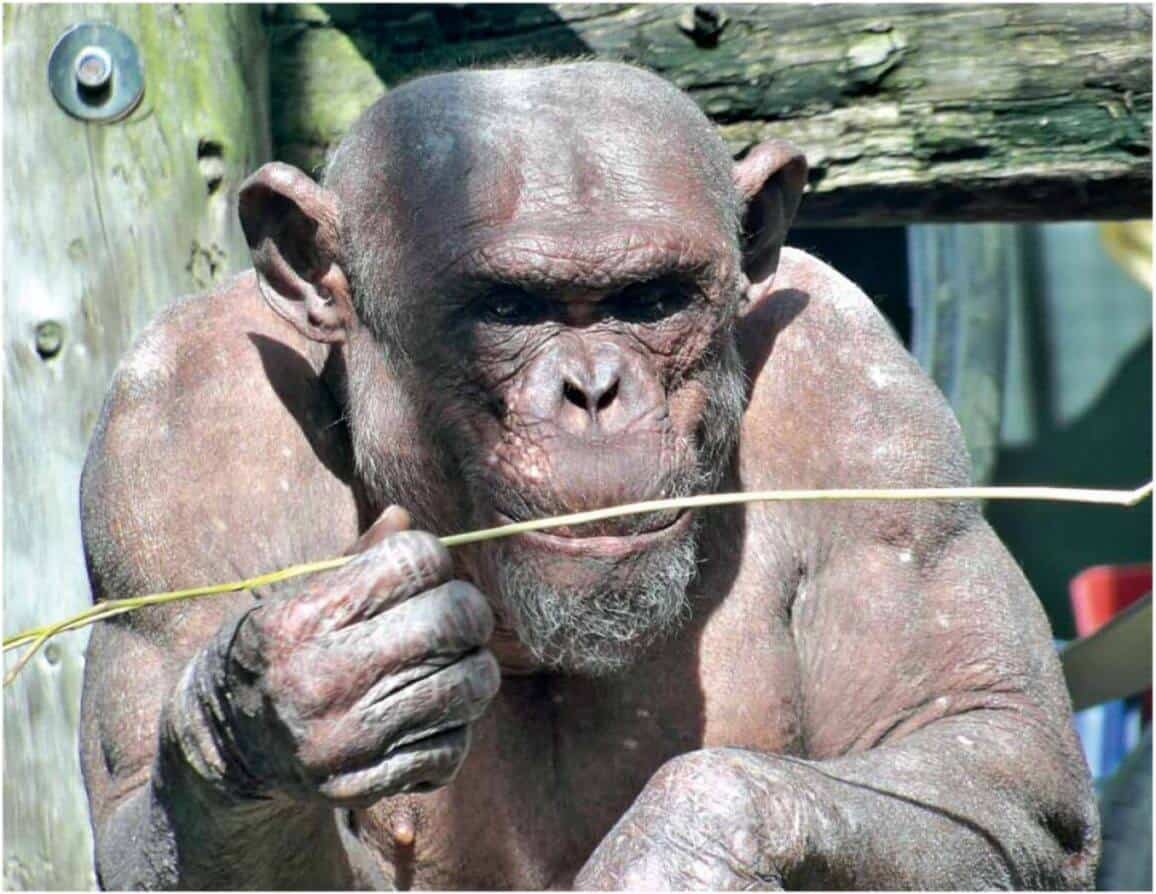
\includegraphics[width=0.8\textwidth]{pictures/chimp.jpg}
    \caption{This is how the chimps look like, I guess...}
    \label{fig:chimp}
\end{figure}


This is eurler's formula: $e^{i\pi} + 1 = 0$ ,

but we can also write it this way:
$$ \lim_{n\to\infty} \left(1 + \frac{1}{n}\right)^{n}= 
\lim_{n\to\infty} \left(\frac{n}{\sqrt[n]{n!}}\right)$$
or this way : 
$$e = \sum_{n=0}^{\infty} \frac{1}{n!}$$
This is famous "geometric mean": $G = \sqrt[n]{x_1 * x_2 * x_3 *....* x_n}$
\pageref{fig:chimp}
\newpage
\begin{Huge}
\begin{center}
\title{Lista Numerowana}
\end{center}
\end{Huge}
\begin{enumerate}
    \item pierwsza linia,
    \item druga linia,
    \item trzecia linia,
\end{enumerate}

\begin{Huge}
\begin{center}
    \title{Lista Nienumerowana}
\end{center}
\end{Huge}
\begin{itemize}
    \item pierwsza linia
    \item druga linia
    \item trzecia linia
\end{itemize}

Here I will write \begin{Huge}BIG LETTERS\end{Huge} alongside the \begin{tiny}small ones\end{tiny} some of which are \textbf{BOLDENED}  and some are \textit{ITALICIZED} and some just \texttt{LOOK WEIRD}
\begin{center}
Additionally I can put this text to the center,
\end{center}
\begin{flushright}
This one to the right,
\end{flushright}
\begin{flushleft}
and that one to the left.
\end{flushleft}

\begin{table}[]
    \centering
    \begin{tabular}{l|c|r}
         \hline
         Name     & Age & Hobby\\
         \hline
         Boguslaw & 19  & Bridge\\
         \hline
         Georgio  & 18  & Racing\\
         \hline
         Jacob    & 20  & Sleeping\\
         \hline
    \end{tabular}
    \caption{Table of Hobbies}
    \label{tab:my_label}
\end{table}

\newpage
\begin{Large} Spis Treści(referencje): \end{Large}
\begin{enumerate}
\item chimp - page: \pageref{fig:chimp}
\item table - page: \pageref{tab:my_label}
\end{enumerate}